\chapterimage{stairs}
\chapter{Quantization}\label{sec:quantization}

This chapter presents quantization as a key stage of lossy compression pipelines,
and introduces some of the main examples used in practice.

\section{Symbol grouping}

Consistent with Chapters~\ref{sec:data:media} and~\ref{sec:info:elements},
digital data can be regarded as a collection of samples from a
finite \concept{alphabet} \alphabet.
%
When those data represent a \concept{physical} signal such as light intensity
or sound pressure, the more elements in \alphabet, the more precise that representation
can be.

\begin{center}
\begin{tikzpicture}
\begin{axis}[
    width=14cm,
    height=4cm,
    domain=0:2*pi,
    samples=500,
    axis lines=none,
    ticks=none,
    xlabel={}, ylabel={},
]

% Original sine wave (2 cycles)
\addplot[
    thick,
    color1,
    domain=0:2*pi,
    samples=500,
] {sin(deg(2*x))};

% Quantized sine wave (8 levels), step function
\addplot[
    thick,
    color2,
    const plot,
    no markers,
    domain=0:2*pi,
    samples=500,
]
({x}, {round((sin(deg(2*x)) + 1)*3.5)/3.5 - 1});

\end{axis}
\end{tikzpicture}

\end{center}

\conceptRef{quantization}{Quantization} is a process that splits the input
alphabet into groups, and outputs the same \concept{quantization index}
for all elements of the same group. This can be expressed as a \concept{scalar}
function:

\begin{center}
\begin{minipage}{0.4\linewidth}
\begin{eqnarray*}
Q:\alphabet & \longrightarrow & \otheralphabet\\
  x & \longrightarrow & Q(x).
\end{eqnarray*}
\end{minipage}
\end{center}

An example quantizer function is shown next:

\begin{center}
\alphabet 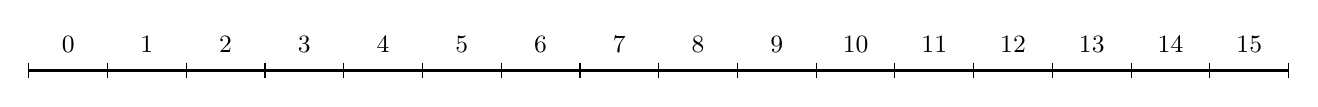
\begin{tikzpicture}
% Total segment length and number of divisions
\def\length{16}  % cm
\def\divisions{16}
\def\step{\length/\divisions}

% Draw main segment
\draw[thick] (0,0) -- (\length,0);

% Draw division ticks
\foreach \i in {0,...,\divisions} {
    \draw[thin] ({\i*\step},0.1) -- ({\i*\step},-0.1); % Vertical tick mark
}

% Draw interval labels centered between ticks
\foreach \i in {0,...,15} {
    \node[anchor=south] at ({(\i+0.5)*\step},0.1) {\small \i};
}

\end{tikzpicture}
\\
$\big\downarrow$\\
\otheralphabet 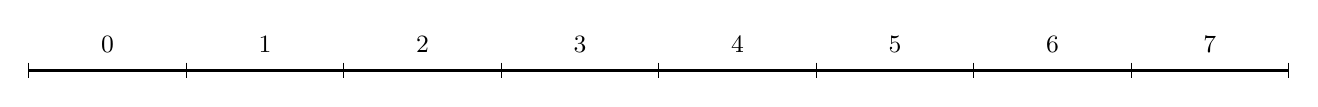
\begin{tikzpicture}
% Total segment length and number of divisions
\def\length{16}  % cm
\def\divisions{16}
\def\step{\length/\divisions}

\draw[thick] (0,-1) -- (\length,-1);

\foreach \i in {0,...,8} {
    \draw[thin] ({\i*\step*2},-0.9) -- ({\i*\step*2},-1.1); % Vertical tick mark
}
\foreach \i in {0,...,7} {
    \node[anchor=south] at ({(\i+0.5)*\step*2},-0.9) {\small \i};
}

\end{tikzpicture}

\end{center}


Applying quantization to the symbols produced by a source \source
can be regarded as having a new source $\othersource=Q(\source)$ that produces
symbols (quantization indices) from smaller alphabet $\otheralphabet=Q(\alphabet)$.
%
The new source $\othersource$ has a different \concept{probability distribution}.
In general, $\entropy(\othersource) < \entropy(\source)$, which is why quantization
is included in data compression pipelines.

Along with a quantization function $Q$, one needs to define a
\mbox{\concept{dequantization}} function $Q^{-1}:\otheralphabet \longrightarrow \alphabet$
that decides the \concept{reconstruction point} of each quantization interval.
This reconstruction point is normally one of the input symbols that
is quantized to that interval, \ie, $Q^{-1}(y) \in \{x \in \alphabet : Q(x) = y\}$.

After a symbol is quantized,
one can only know what group that symbol belongs to, but not which symbol exactly.
%
Therefore, quantization is a \conceptRef{lossy compression}{lossy} process (often the only one in
a lossy compression pipeline~\cite[\S 3.1]{taubman2002jpeg2000}).
%
Once $Q$ and $Q^{-1}$ are defined, one can compute the expected quadratic error as
$
E[\left( X - Q^{-1}(Q(X))\right)^2] = \sum_{\sigma \in \alphabet} P(\sigma) \left(\sigma - Q^{-1}(Q(\sigma))\right)^2.
$


\section{Popular quantizers}\label{sec:quantization:examples}

The most simple, nontrivial quantizer is \concept{uniform scalar quantization}~\cite[\S 9.4]{sayood_introduction}.
As the name implies,
all quantization intervals have the same length. This length is often referred to as the \concept{quantization step},
\aka\ \concept{qstep}, and typically denoted $\Delta$.
%
In spite of its simplicity, uniform quantization is close to optimal (in terms of \concept{rate-distortion})
for high enough rates (\ie, for small enough intervals)~\cite[\S 3.2.4, Fig.~3.5]{taubman2002jpeg2000}.
%
When signed inputs are considered, there are two possibilities:
\begin{itemize}
\item \conceptRef{midrise quantizer}{Midrise}~\cite[Fig.~9.3]{sayood_introduction}: when $\nexists y \in \otheralphabet \ :\ Q^{-1}(y) = 0$, and
\item \conceptRef{midtread quantizer}{Midtread}~\cite[Fig.~9.5]{sayood_introduction}: when $\exists y \in \otheralphabet \ :\ Q^{-1}(y) = 0$.
\end{itemize}

One very desirable feature of compression systems is the possibility of sending some
data first (which enables the reconstruction at a certain quality),
and later on sending more data to enhance that quality. This feature is called
\concept{progressive transmission} (or progressive reconstruction, depending on the point of view).
%
An efficient way of achieving this is by using \concept{embedded quantization}:
\begin{itemize}
\item To build an embedded quantizer, a quantizer $Q_1$ is defined on the original alphabet $\alphabet$.
After that, a second quantizer $Q_2$ is defined on the quantization intervals
produced by $Q_1$, \ie, on $Q_1(\alphabet)$. As a result, the quantization intervals
defined by $Q_1$ are contained \mbox{--\conceptRef{embedded quantization}{embedded}--}
in $Q_2$'s. This process is repeated until the last (and coarsest) quantizer $Q_D$
is defined on the intervals given by $Q_{D-1}(Q_{D-2}(\cdots Q_1(\alphabet)))$.
\vspace{0.1cm}

\item To apply an embedded quantizer, the emitter applies the coarsest quantizer $Q_D$ first.
The resulting quantization intervals can be transmitted, and used for reconstruction
by the receiver. After that, for each transmitted quantization index, additional information
can be send so that the receiver knows to which of $Q_{D-1}$'s intervals the original
sample belongs.
\vspace{0.1cm}

\item The most common embedded quantizer is one where each $Q_i$ is a uniform scalar
quantizer with qstep $2$, and the last quantizer has $2$ quantization intervals~\cite[\S 3.2.6]{taubman2002jpeg2000}.
In this case, a single bit is sufficient to select the first quantization interval.
Each additional bit allows selecting an interval of the next quantizer, effectively
halving the qstep. This process is equivalent to successively transmitting the
\conceptRef{bitplane}{bitplanes} of the original data, from most to least significant.
%
These bitplanes can (and generally are) entropy coded with a \concept{binary entropy coder}.
%
Note that embedding is not restricted to uniform scalar quantizers,
and generalizations have been described~\cite{auli_geq}.
\end{itemize}

Nothing forces us to have all quantization intervals have the same size. In fact,
\conceptRef{non-uniform quantization}{non-uniform quantizers} are required to achieve
optimality in the general case.
\begin{itemize}
\item One very elegant example of a non-uniform scheme is \concept{deadzone quantization}~\cite[Eq.~3.30]{taubman2002jpeg2000}. Usually, this approach is constructed as a uniform quantizer
with an enlarged (\eg, twice the size), zero-centered interval. This case is called a
\concept{deadzone uniform scalar quantizer} -- but it is not actually uniform as defined above
because of that enlarged central interval. This approach yields enhanced performance
for zero-mean probability distributions, which is often the case after prediction (see Chapter~\ref{sec:prediction}) and transforms such as the DWT (see Chapter~\ref{sec:transforms}).
\vspace{0.1cm}

\item If the probability distribution of the source \source is known, one can use this information
to design the quantizer that minimizes $E[\left(X - Q^{-1}(Q(X))\right)^2]$.
The \concept{Lloyd-Max algorithm}~\cite[\S 3.2.1]{taubman2002jpeg2000},~\cite[\S 9.6.1]{sayood_introduction} can be used for this purpose,
which yields optimal quantizers (in the rate-distortion sense) assuming no entropy coding
is applied after quantization.
%
For the case where entropy coding \textit{is} applied, there exists a generalized version
of this algorithm~\cite[\S 3.2.3]{taubman2002jpeg2000},~\cite[\S 9.7.1]{sayood_introduction}.

\end{itemize}



%
% * **Non-uniform scalar quantization**. Nothing forces us to make all quantization intervals the same size. If we don't, then we are applying *non-uniform* scalar quantization, which can sometimes yield better results than scalar quantization. There exist iterative algorithms that output optimal non-uniform designs given a source's symbol probability distribution: Lloyd-Max if no entropy coding is applied after quantization (R1 9.6.1), and entropy-constrained Lloyd-Max if entropy coding is applied to the quantization indices (R1 9.7, R3).
%
% * **Vector quantization**. Instead of quantizing each input symbol individually (x -> Q(x)), we can quantize multiple symbols at a time (x1,x2,...,xV -> Q(x1,x2,...,xV). In this case, inputs (x1,x2,...,xV) are called *vectors* and the process is referred to as *vector quantization*. As in the scalar case, multiple inputs are assigned to the same quantization interval. On the other hand, the dequantization function Q⁻¹ reconstructs a vector of V symbols per quantization interval. Vector quantization tends to produce better rate-distortion trade-offs than scalar quantization, but at the cost of higher computational complexity (R1 10.3). There exist algorithms for designing efficient vector quantization designs (R1 10.4).


\section*{Further reading and practice}
\vspace{0.25cm}
\begin{itemize}
\item Sayood's book~\cite{sayood_introduction} is an excellent companion for this section,
particularly \S 9.1--9.4, 9.6 and 9.7.
\item A generalization of embedded quantization was described in detail in~\cite{auli_geq}.
\item Another example of a non-uniform quantizer designed for a particular purpose
can be found in~\cite{hernandez_analysis}.
\item Taubman and Marcellin's book extends the contents of this Chapter including
non-scalar quantizers~\cite[\S 3.4]{taubman2002jpeg2000} and Trellis Quantization~\cite[\S 3.5]{taubman2002jpeg2000}.
\end{itemize}

\begin{exercise}
Mathematically define the quantization function $Q$ and its corresponding reconstruction
function $Q^{-1}$ for each of the main types mentioned in the chapter.
\end{exercise}

\begin{exercise}
A source \source produces elements from an alphabet \alphabet with entropy \entropy(\source).
We apply a uniform scalar quantizer with step $2$. What is the minimum and maximum
entropy of the output?
\end{exercise}

\begin{exercise}
Given a source \source and a quantization function $Q$,
how would you choose the optimal reconstruction point for each
quantization interval?
\end{exercise}

\begin{exercise}
What's the relation between $\entropy(Q(\source))$ and $\entropy(Q^{-1}(Q(\source)))$?
\end{exercise}

\begin{exercise}
Looking only at the value distributions (histograms), how would you identify the
original data from a source \source, the quantization indices produced by a quantizer $Q$,
and the reconstructed data $Q^{-1}(Q(\source))$?
\end{exercise}

\begin{exercise}
Split the mandrill image sample (\url{mandrill-u8be-3x512x512.raw}) into its
bitplane constituents. What qualitative differences do you observe between the
most and least significant bitplanes?
\end{exercise}



